\documentclass{report}
\usepackage{tikz}
\begin{document}
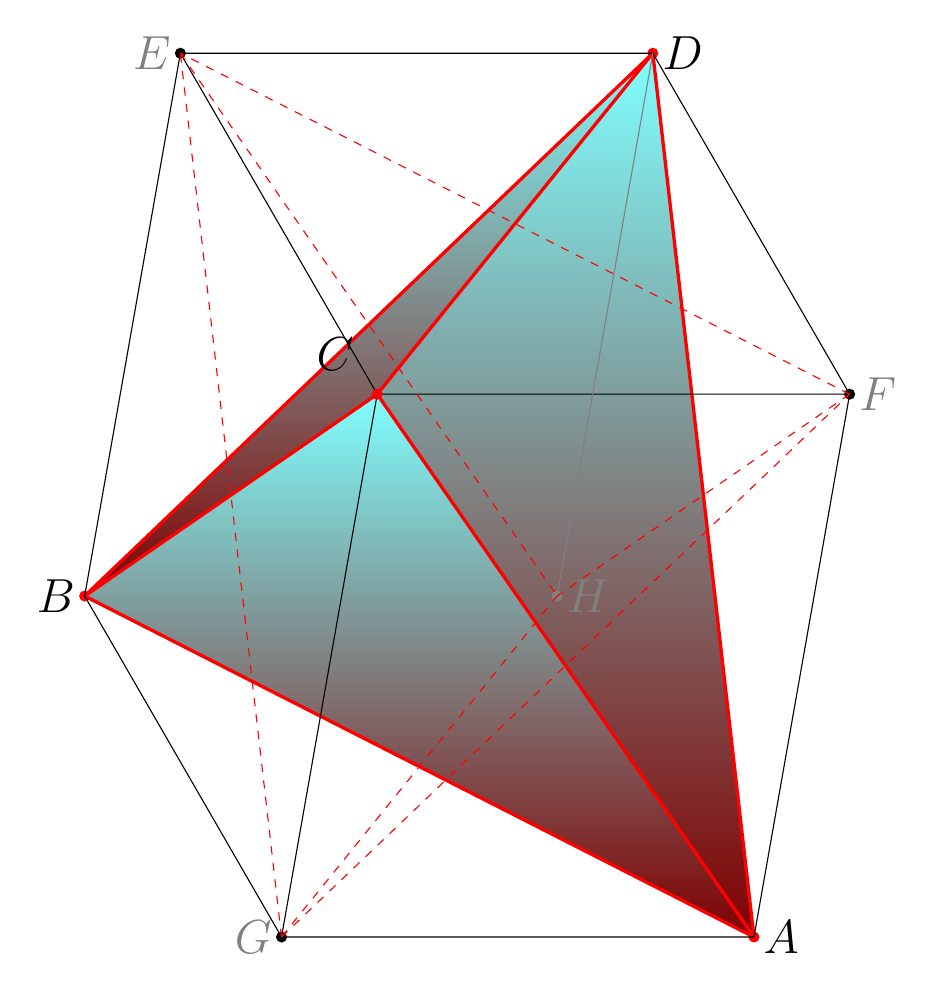
\begin{tikzpicture}[font=\LARGE]
\def \tta{ -10.00000000000000 }
\def \k{    -3.00000000000000 }
\def \l{     6.00000000000000 }
\def \d{     5.00000000000000 }
\def \h{     7.00000000000000 }
\coordinate (A) at (0,0);
\coordinate (B) at ({-\h*sin(\tta)},{\h*cos(\tta)});
\coordinate (C) at ({-\h*sin(\tta)-\d*sin(\k*\tta)},
                    {\h*cos(\tta)+\d*cos(\k*\tta)});
\coordinate (D) at ({-\d*sin(\k*\tta)},{\d*cos(\k*\tta)});
\coordinate (Ap) at (\l,0);
\coordinate (Bp) at ({\l-\h*sin(\tta)},{\h*cos(\tta)});
\coordinate (Cp) at ({\l-\h*sin(\tta)-\d*sin(\k*\tta)},
                     {\h*cos(\tta)+\d*cos(\k*\tta)});
\coordinate (Dp) at ({\l-\d*sin(\k*\tta)},{\d*cos(\k*\tta)});
\fill[black]  (A) circle [radius=2pt];
\fill[red]    (B) circle [radius=2pt];
\fill[black]  (C) circle [radius=2pt];
\fill[red]    (D) circle [radius=2pt];
\fill[red]   (Ap) circle [radius=2pt];
\fill[black] (Bp) circle [radius=2pt];
\fill[red]   (Cp) circle [radius=2pt];
\fill[black] (Dp) circle [radius=2pt];
\filldraw[draw=red,bottom color=red!50!black, top color=cyan!50]
  (B) -- (Cp) -- (D);
\filldraw[draw=red,bottom color=red!50!black, top color=cyan!50]
  (B) -- (D)  -- (Ap);
\filldraw[draw=red,bottom color=red!50!black, top color=cyan!50]
  (B) -- (Cp) -- (Ap);
\draw[red,-,very thick] (Ap) --  (D)
                        (Ap) --  (B)
                        (Ap) -- (Cp)
                        (B)  --  (D)
                        (Cp) --  (D)
                        (B)  -- (Cp);
\draw [-,thin] (B)  --  (A)
               (Ap) -- (Bp)
               (B)  --  (C)
               (D)  --  (C)
               (A)  --  (D)
               (Ap) --  (A)
               (Cp) --  (C)
               (Bp) --  (B)
               (Bp) -- (Cp);
\draw [gray,-,thin] (Dp) -- (Cp);
                    (Dp) --  (D);
                    (Ap) -- (Dp);
\draw (Ap) node [right]           {$A$}
      (Bp) node [right, gray]     {$F$}
      (Cp) node [right]           {$D$}
      (C)  node [left,gray]       {$E$}
      (D)  node [left]            {$B$}
      (A)  node [left,gray]       {$G$}
      (B)  node [above left=+5pt] {$C$}
      (Dp) node [right,gray]      {$H$};
\fill[red]   (B) circle [radius=2pt];
\fill[gray] (Dp) circle [radius=2pt];
\draw[red,-,dashed, thin] (A)  -- (Dp)
                          (A)  -- (Bp)
                          (A)  --  (C)
                          (Bp) -- (Dp)
                          (C)  -- (Dp)
                          (Bp) --  (C);
\end{tikzpicture}
\end{document}
